% figure to illustrate match a substring in a text.
\ifdefined\includetikz\relax \else
%\documentclass{standalone}
\documentclass{article}
\usepackage{tikz}
\usepackage{amsmath}
\usetikzlibrary{matrix,backgrounds,positioning}
\begin{document}
\fi

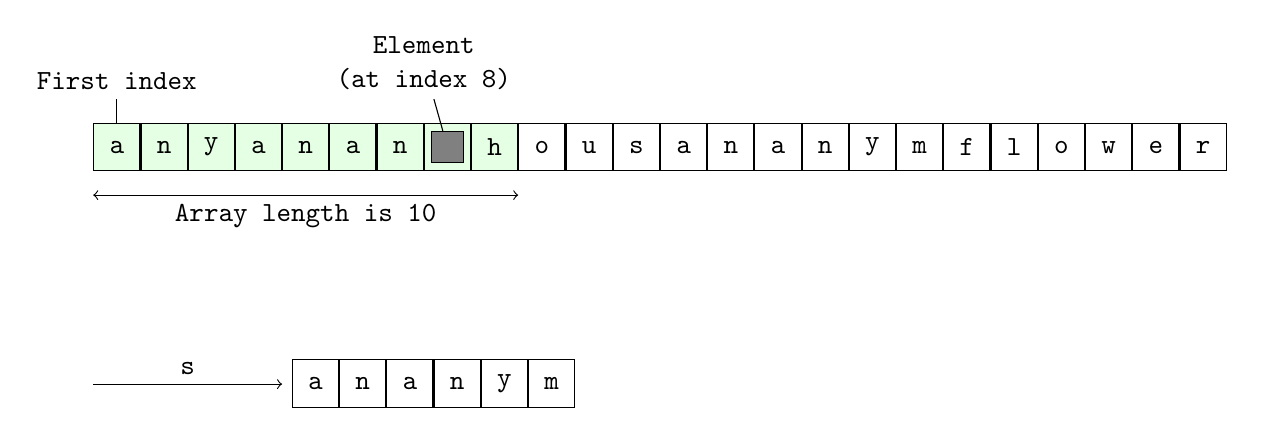
\begin{tikzpicture}[font=\ttfamily,
scale=1,
array/.style={matrix of nodes,
              nodes={draw, align=center, anchor=south, minimum height = 4ex, text width=1em}
              %column sep=-\pgflinewidth,
              %row sep=0.5mm,
              %nodes in empty cells
              %row 1/.style={nodes={draw=none, fill=none, minimum size=5mm}},
              %row 1 column 1/.style={nodes={draw}}
              }]

%any ananthous ananym flower
\matrix[array] (array) {
a & n & y & & a & n & a & n & t & h & o & u & s & & a & n & a & n & y & m & & f & l & o & w & e & r \\};

%ananym
\matrix[array,
  yshift=-3cm,
  right=0 of array-1-5] (myptn) {
a & n & a & n & y & m \\};

% offset s
\draw[->] ([yshift=-2.7cm]array-1-1.south west) -- node[above] {s} ([yshift=-2.7cm]array-1-5.south east);

\node[draw, fill=gray, minimum size=4mm] at (array-1-9) (box) {};

\begin{scope}[on background layer]
\fill[green!10] (array-1-1.north west) rectangle (array-1-10.south east);
\end{scope}

\draw[<->]([yshift=-3mm]array-1-1.south west) -- node[below] {Array length is 10} ([yshift=-3mm]array-1-10.south east);

\draw (array-1-1.north)--++(90:3mm) node [above] (first) {First index};
%\draw (array-1-10.east)--++(0:3mm) node [right]{Indices};
\node [align=center, anchor=south] at (array-1-9.north west|-first.south) (8) {Element\\ (at index 8)};
\draw (8)--(box);
%
\end{tikzpicture}

\ifdefined\includetikz\relax \else
\end{document}
\fi
